\documentclass{beamer}
\usetheme{metropolis}
\usepackage{graphicx}
\graphicspath{{../../latex/images/}}
\usepackage{boolexpr}
\usepackage{kpfonts}
\usepackage{caption}
\usepackage{wrapfig}
\usepackage{tkz-graph}
\usepackage{tikz}
\usepackage[labelformat=empty]{caption}
\usepackage[official]{eurosym}

\usepackage{minted}

\usepackage{siunitx}

\usepackage[math]{iwona}
\usepackage{scalerel}
\def\lVert{\mid\!\mid}
\def\rVert{\mid\!\mid}

\usepackage[normalem]{ulem}
\usepackage{mathtools}

\usepackage{../../latex/custom}
\usepackage{amsfonts}

\newcommand{\expe}[2]{\la #1, #2 \ra}

\usepackage{framed}

\newcommand\Wider[2][3em]{%
\makebox[\linewidth][c]{%
  \begin{minipage}{\dimexpr\textwidth+#1\relax}
  \raggedright#2
  \end{minipage}%
  }%
}

\newcommand{\aeur}{\alpha_\text{\euro}}
\newcommand{\adol}{\alpha_\$}
\newcommand{\apou}{\alpha_\text{\pounds}}

\title{Julia for Operations Research}
\date{October 22, 2019}
\author{Beno\^it Legat (UCLouvain)}
\institute{Petit D\'ej' de l'I\&D, N-SIDE}

\makeatletter
\let\@@magyar@captionfix\relax
\makeatother
\begin{document}
  \maketitle

  \begin{frame}
    \frametitle{JuMP: optimization without compromise}
    \begin{tabular}{p{0.45\textwidth}|p{0.45\textwidth}}
      \textbf{Basic} & \textbf{Advanced}\\
      \hline
      Easy to install, setup, use & Fast\\
      \hline
      Simple to do simple things & Consistent interface for advanced features\\
      \hline
      Solver-independent interface & Give access to solver-specific features\\
      \hline
      Transparently circumvent solver limitations & Allow direct contact with solver\\
      \hline
      Reliability \& consistency & Distributed ecosystem\\
    \end{tabular}
  \end{frame}

  \begin{frame}
    \tableofcontents
  \end{frame}

\section{Usability \& Efficiency}

  \begin{frame}
    \frametitle{Julia language ambition}
    Initial blog post from 2012:
    \begin{center}
      \emph{
We want the speed of C with the dynamism of Ruby. We want a language that's homoiconic, with true macros like Lisp, but with obvious, familiar mathematical notation like Matlab. We want something as usable for general programming as Python, as easy for statistics as R, as natural for string processing as Perl, as powerful for linear algebra as Matlab, as good at gluing programs together as the shell. Something that is dirt simple to learn, yet keeps the most serious hackers happy. We want it interactive and we want it compiled.

(Did we mention it should be as fast as C?)
      }
    \end{center}
  \end{frame}

  \begin{frame}[fragile]
    \frametitle{Multiple dispatch}
    \begin{minted}{Julia}
function power_by_squaring(x, p::Integer)
    ...
end
^(x::Number, p::Integer) = power_by_squaring(x, p)
^(x::AbstractMatrix, p::Integer) = power_by_squaring(x, p)
^(x::BigInt, p::Integer) = MPZ.pow_ui(x, p)
^(x::Float64, p::Float64) = ccall("llvm.pow.f64", ...)
^(x::Float32, p::Float32) = ccall("llvm.pow.f32", ...)
    \end{minted}

    Julia compiler compiles each method \emph{Just-In-Time} to LLVM IR.
    LLVM IR is then compiled to machine code.
    The LLVM IR to machine code layer is shared with all languages relying on LLVM (e.g. Clang, Scala Native).

    \emph{Multiple dispatch} allows both \alert{abstraction} and \alert{specialization}.
  \end{frame}

  \begin{frame}[fragile]
\frametitle{Metaprogramming}
\begin{minted}{Julia}
@constraint(model, [i = 1:3, j = 1:i; isodd(i + j)],
            i*x + j*y + z*(i+j) == i * j)
\end{minted}
\begin{minted}{Julia}
container(((i, j)->begin
  expr0 = Val{false}()
  expr1 = _destructive_add_with_reorder!(expr0, i, x)
  expr2 = _destructive_add_with_reorder!(expr1, j, y)
  expr3 = _destructive_add_with_reorder!(expr2, z, i)
  expr4 = _destructive_add_with_reorder!(expr3, z, j)
  expr5 = _destructive_add_with_reorder!(expr4, -1.0,
                                         i, j)
  con = build_constraint(expr5, EqualTo(0.0))
  JuMP.add_constraint(model, con, "")
end, nested(()->1:3, (i,)->1:i;
            condition=(i, j)->isodd(i + j)))
\end{minted}
  \end{frame}


\section{Consistency}

  \begin{frame}
    \frametitle{From macros to solver}
    \begin{center}
      \emph{A convenient UI should not hide a hacky low-level interface.}
    \end{center}
    \begin{itemize}
      \item JuMP macros transformed at parsing time to JuMP function calls.
      \item JuMP function calls redirect to MOI function calls.
      \item MOI function calls redirect to solver API calls.
    \end{itemize}
  \end{frame}

  \begin{frame}
    \frametitle{Enforcing consistency of solver MOI interfaces}
    \begin{itemize}
      \item Abstract Model and Optimizer types.
      \item Detailed documentation.
      \item Extensive test suite run by every solvers and MOI internal models.
      \item Utilities for sanity checks, duplicate removal in functions, get fallbacks...
    \end{itemize}
  \end{frame}

\section{Flexibility}

  \begin{frame}[fragile]
    \frametitle{MathOptInterface (MOI)}
    \begin{itemize}
      \item \verb|add_variable(model)|, \verb|add_constrained_variable(model, set)|.
      \item \verb|add_constraint(model, func, set)|, e.g. $2x + 3y = 1$ $\to$ (\verb|2*x + 3*y|)-in-\verb|EqualTo(1.0)|.
      \item \verb|set|, \verb|get| attributes, e.g., \verb|ObjectiveFunction|, \verb|HeuristicCallback|.
      \item \verb|submit| submittables, e.g., \verb|HeuristicSolution|.
    \end{itemize}
    Extensible framework:
    \begin{itemize}
      \item \alert{Generic} on attribute, function and set types. New ones can be defined \alert{independently}.
      \item Solver-\alert{specific} features easily exposed to JuMP/MOI users through \alert{custom} attributes, e.g. solver specific callbacks.
      \item Expose \alert{specialized} problem structure easily through \alert{custom} functions, sets (e.g. indicator constraints, complementarity constraints, ...).
    \end{itemize}
  \end{frame}

  \begin{frame}[fragile]
    \frametitle{Solver-specific callbacks}
\begin{minted}{Julia}
MOI.set(model, GLPK.CallbackFunction(),
	(cb_data) -> begin
  reason = GLPK.ios_reason(cb_data.tree)
  if reason == GLPK.IHEUR
    ...
    accepted = MOI.submit(
      model, MOI.HeuristicSolution(cb_data), ...)
  elseif reason == GLPK.ICUTGEN
    ...
    MOI.submit(model, MOI.UserCut(cb_data), ...)
  end
end)
\end{minted}
  \end{frame}

  \begin{frame}[fragile]
    \frametitle{Solver-independent callbacks}
\begin{minted}{Julia}
MOI.set(model, MOI.HeuristicCallback(),
	(cb_data) -> begin
  ...
  accepted = MOI.submit(
    model, MOI.HeuristicSolution(cb_data), ...)
end)
\end{minted}
\begin{minted}{Julia}
MOI.set(model, MOI.UserCutCallback(),
	(cb_data) -> begin
  ...
  MOI.submit(model, MOI.UserCut(cb_data), ...)
end)
\end{minted}
  \end{frame}


\section{Modularity}

  \begin{frame}[fragile]
    \frametitle{Breaking down the MOI backend}
    Distinction between:
    \begin{itemize}
      \item Unsupported constraints, attributes: resolved by \emph{bridges}.
      \item Unsupported modification: resolved by a \emph{caching layer}.
    \end{itemize}
    MOI.Utilities.CachingOptimizer has 2 modes:
    \begin{itemize}
      \item Automatic: Automatically empty optimizer when a modification is not supported and re-copy at optimize.
      \item Manual: Need to manually reset optimizer or an error is thrown.
    \end{itemize}
    JuMP has 3 modes:
    \begin{itemize}
      \item Direct: No cache nor bridge (can be added manually though).
      \item Automatic: Cache in AUTOMATIC mode and bridges.
      \item Manual: Cache in manual mode and bridges.
    \end{itemize}
  \end{frame}

  \begin{frame}{Semidefinite programming}
    \begin{align*}
      \mini_{Q \in \SymK} \quad & \la C, Q \ra & \maxi_{y \in \R^n} \quad & \la b, y \ra\\
      \subtoq & \la A_i, Q \ra = b_i & \subtoq & \sum_i A_i y_i \preceq C\\
        & Q \succeq 0
    \end{align*}
    \textbf{File format}: SDPA

    \textbf{Solvers}: CSDP, SDPA, DSDP, SDPLR, ...

    \textbf{Variables}: $Q$ block diagonal, nonnegative scalar variables ($1 \times 1$ blocks) or SDP matrices.

    \textbf{Constraints}: Affine equations.
  \end{frame}

\begin{frame}{Interval constraint for SDPA}
\Wider[4em]{
  \begin{center}
    \begin{tikzpicture}[xscale=4.5, yscale=2]
      \tikzset{VertexStyle/.style = {}}
      \Vertex[x=1, y=-1, L={$a^\top x + \beta \ge l$}]{G}
      \Vertex[x=2, y=-1, L={$a^\top x + \beta \le u$}]{L}
      \Vertex[x=1, y=-2, L={$A x + b \in \mathbb{R}_+^1$}]{N}
      \Vertex[x=2, y=-2, L={$A x + b \in \mathbb{R}_-^1$}]{P}
      \Vertex[x=1, y=-3, L={$A x + b \in \{0\}^1$}]{Z}
      \Vertex[x=0, y=0, L={$x \le u$}]{VL}
      \Vertex[x=0, y=-1, L={$x \ge l$}]{VG}
      \Vertex[x=0, y=-2, L={$x \in \mathbb{R}_-^1$}]{VP}
      \tikzset{VertexStyle/.style = {
        shape = rectangle,
        draw
      }}
      \Vertex[x=1, y=0, L={$l \le a^\top x + \beta \le u$}]{I}
      \tikzset{VertexStyle/.style = {
        shape = rounded rectangle,
        draw
      }}
      \Vertex[x=2, y=-3, L={$a^\top x = \beta$}]{E}
      \Vertex[x=0, y=-3, L={$x \in \mathbb{R}_+^1$}]{VN}
      \tikzset{EdgeStyle/.style = {->}}
      \Edge[label={flip}](L)(G)
      \Edge[label={flip}](VP)(VN)
      \Edge[label={flip}](VL)(VG)
      \Edge[label={split}](I)(L)
      \Edge[label={split}](I)(G)
      \Edge[label={vectorize}](G)(N)
      \Edge[label={vectorize}](L)(P)
      \Edge[label={scalarize}](Z)(E)
      \Edge[label={slack}](P)(Z)
      \Edge[label={slack}](N)(Z)
      \Edge[label={slack}](N)(VN)
      \Edge[label={slack}](G)(VG)
      \tikzset{EdgeStyle/.style = {->, pos=0.3}}
      \Edge[label={slack}](G)(E)
      \tikzset{EdgeStyle/.style = {->, bend left=22, pos=0.3}}
      \Edge[label={slack}](P)(VP)
      \tikzset{EdgeStyle/.style = {->, bend left=20, pos=0.7}}
      \Edge[label={vectorize}](VL)(VP)
      \tikzset{EdgeStyle/.style = {->, bend left=25, pos=0.8}}
      \Edge[label={slack}](L)(E)
      \tikzset{EdgeStyle/.style = {->, bend right=20, pos=0.3}}
      \Edge[label={vectorize}](VG)(VN)
      \tikzset{EdgeStyle/.style = {->, bend right=25}}
      \tikzset{EdgeStyle/.style = {->, bend right=60, pos=0.2}}
      \Edge[label={slack}](L)(VL)
      \tikzset{EdgeStyle/.style = {->}}
      \Edge[label={flip}](P)(N)
    \end{tikzpicture}
  \end{center}
}
\end{frame}



\begin{frame}
  \frametitle{Bridges directed hypergraph}
  \vspace{-.2cm}
  \begin{block}{Nodes}
    Node for each set $S$ (variable-in-$S$).

    Node for each constraint $F$-in-$S$.

    Node for each objective function $F$.


  \end{block}
  \vspace{-.2cm}
  \begin{block}{Edges}

    For each edge and ingoing node: outgoing nodes are
    \begin{itemize}
        \item variable-in-$S$ created.
        \item constraints $F$-in-$S$ created.
        \item objective $F$ set.
    \end{itemize}
  \end{block}

\end{frame}

\begin{frame}
  \frametitle{Bridges selection}

  \begin{block}{Multiple dispatch ?}
    Can we use multiple dispatch where node types are method signatures ?

    \textbf{No}.
    Several bridge can transform same types.
    Dispatching on more specialized is not accurate.

    Need to guide choice to supported types.
  \end{block}

  \begin{block}{Just in Time (JIT) bridge selection}
    Types $F$ and $S$ are \alert{not limited} to those defined in MOI $\to$
    \alert{infinitely} many nodes.

    Each bridge defined possible \alert{infinitely} many edges.

    Need to be \alert{lazy} and compute bridge selection JIT when
    type first used.
  \end{block}

\end{frame}

\begin{frame}
  \frametitle{Bridge selection algorithm}
  \textbf{Data}: Set of bridges $B$

  \textbf{Invariant}: $d_\mathcal{V}$, $d_\mathcal{C}$, $d_\mathcal{O}$
  are correct when defined.

  Given new type: compute types $T$ where $d$ should be defined with
  Depth First Search (DFS) from the type: $\mathcal{O}(|B|)$.

  Compute $d$ at the types using Bellman-Ford algorithm: $\mathcal{O}(|T| \cdot |B|)$.
\end{frame}

\section{Distributed ecosystem}

\begin{frame}
  \frametitle{MOI extensions}
  MOI wrappers to C/C++ solvers:
  \begin{itemize}
    \item Wrappers developed by JuMP-devs only: BARON, Bonmin, Cbc, CDD, Clp, Couenne, CPLEX, CSDP, ECOS, FICO Xpress, GLPK, Gurobi, Ipopt, SCS, SDPA, SDPT3, SeDuMi, Tulip, PATH
    \item Co-developed with solver developers: Artelys Knitro, CDCS, MOSEK, NLopt, OSQP, SCIP
  \end{itemize}
  Pure Julia solvers:
  \begin{itemize}
    \item COSMO, ProxSDP, Tulip, Hypatia
  \end{itemize}
  Pure Julia \emph{meta}-solvers:
  \begin{itemize}
    \item Juniper, Alpine, Pavito, Pajarito, Coluna, Dualization
  \end{itemize}
\end{frame}

\begin{frame}
  \frametitle{JuMP extensions}
  Polynomial optimization:
  \begin{itemize}
    \item With \alert{polynomials}: MomentOpt, PolyJuMP, SumOfSquares
    \item With \alert{sets}: Polyhedra, SetProg
    \item \alert{Parametrized}: ParameterJuMP, Parametron
    \item \alert{Structured}: BlockDecomposition, StructJuMP
    \item \alert{Stochastic}: SDDP, StochDynamicProgramming, StructDualDynProg
    \item \alert{Multi-objective}: MultiJuMP, vOptSolver
    \item PowerModels, BilevelOptimization, JuMPChance, JuMPeR, Convex, NLOptControl
  \end{itemize}
\end{frame}

\begin{frame}
  \frametitle{Annual JuMP-dev Workshop}
  \begin{columns}
    \begin{column}{0.5\textwidth}
  \begin{center}
    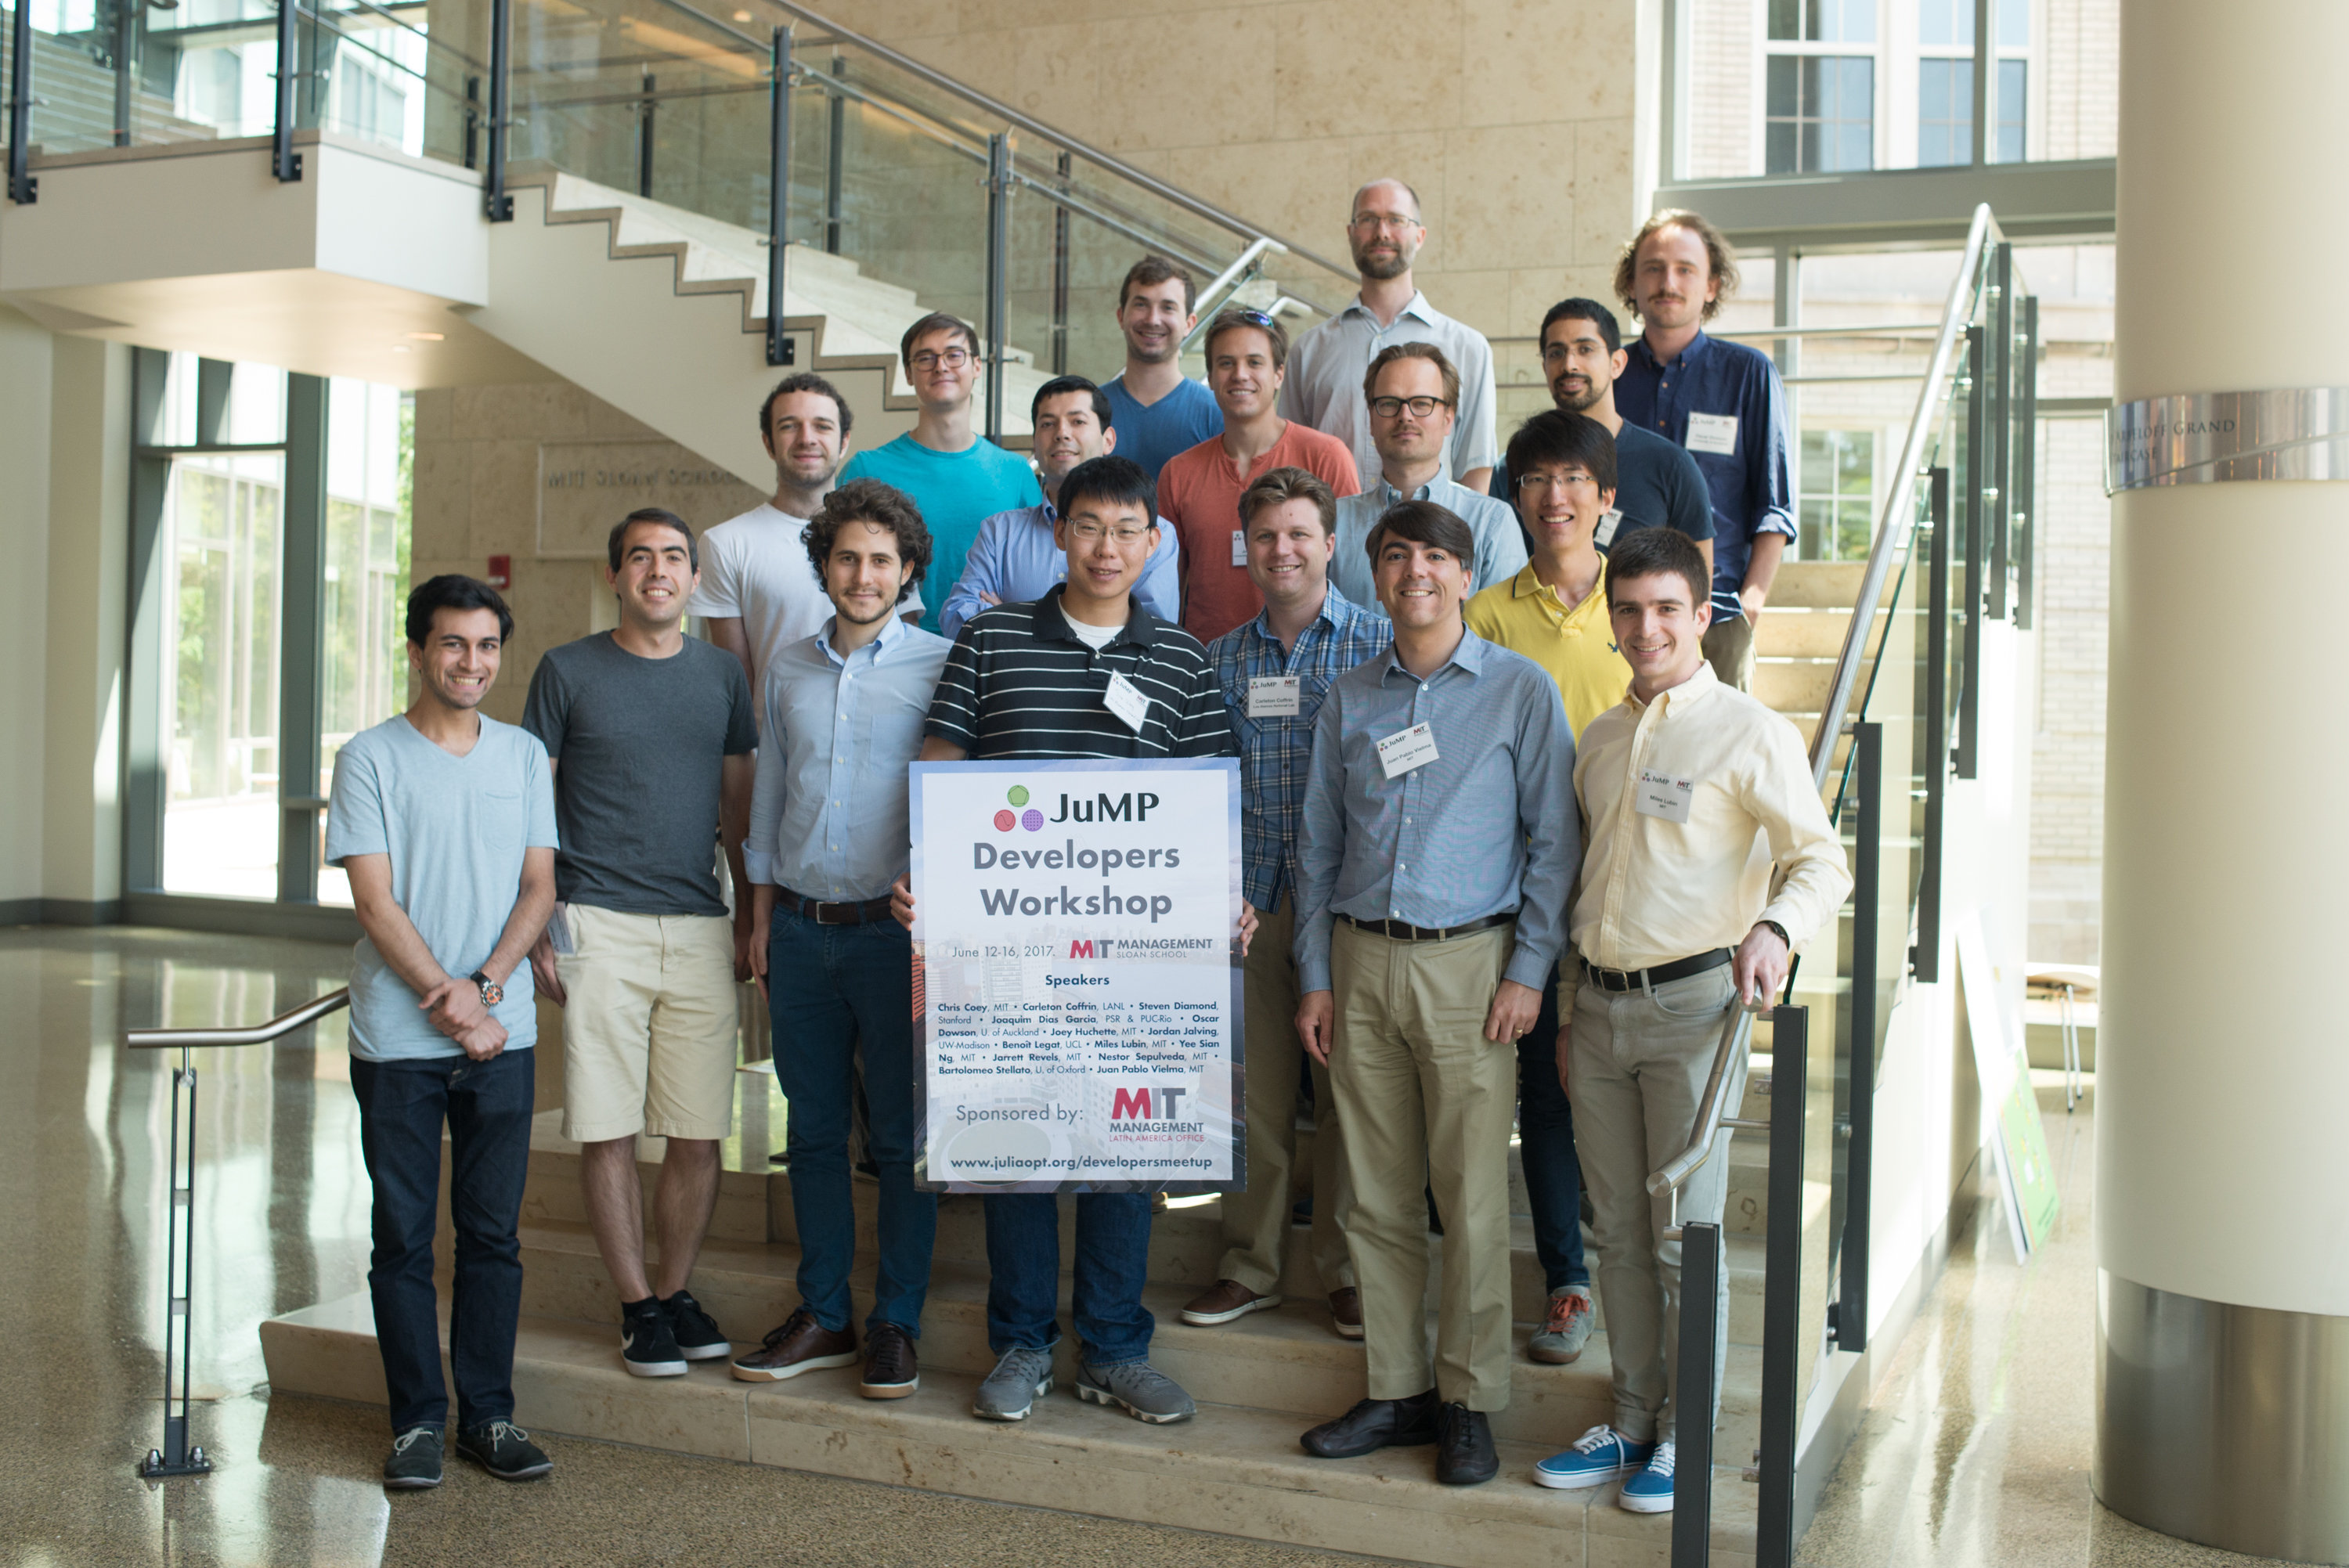
\includegraphics[width=0.8\textwidth]{../../latex/images/JuMP-dev_2017.jpg}
    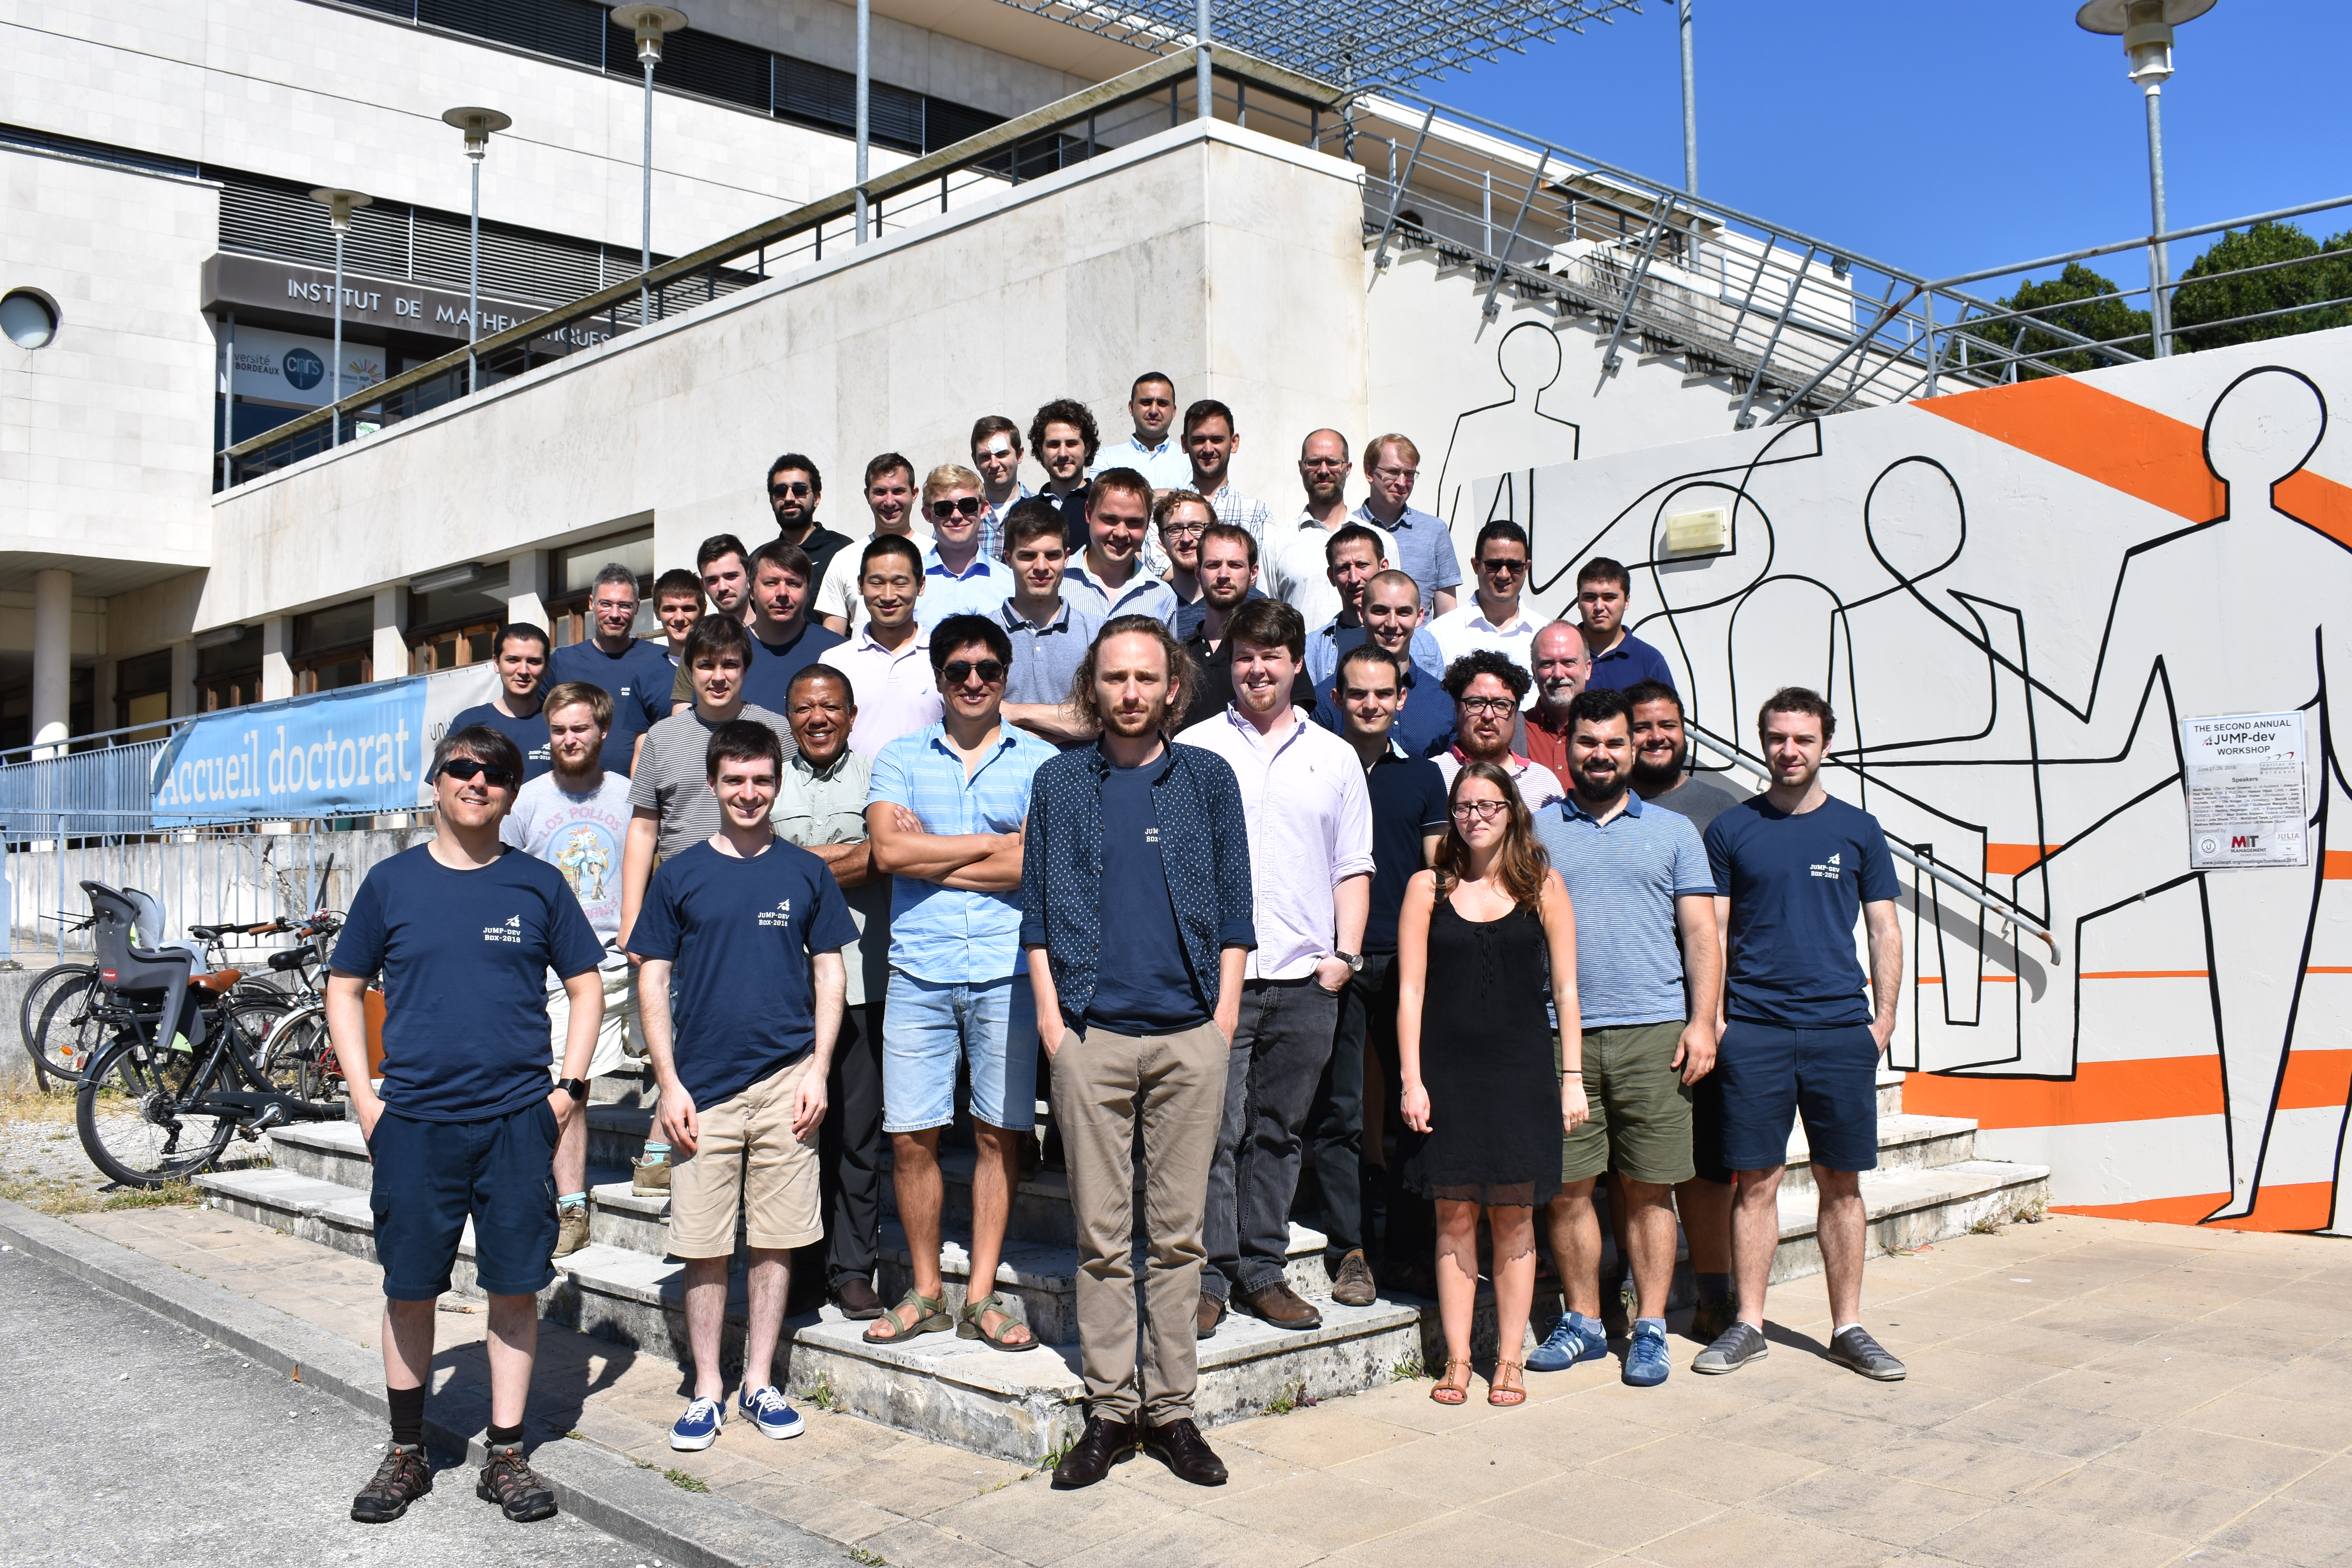
\includegraphics[width=0.8\textwidth]{../../latex/images/JuMP-dev_2018.jpg}
    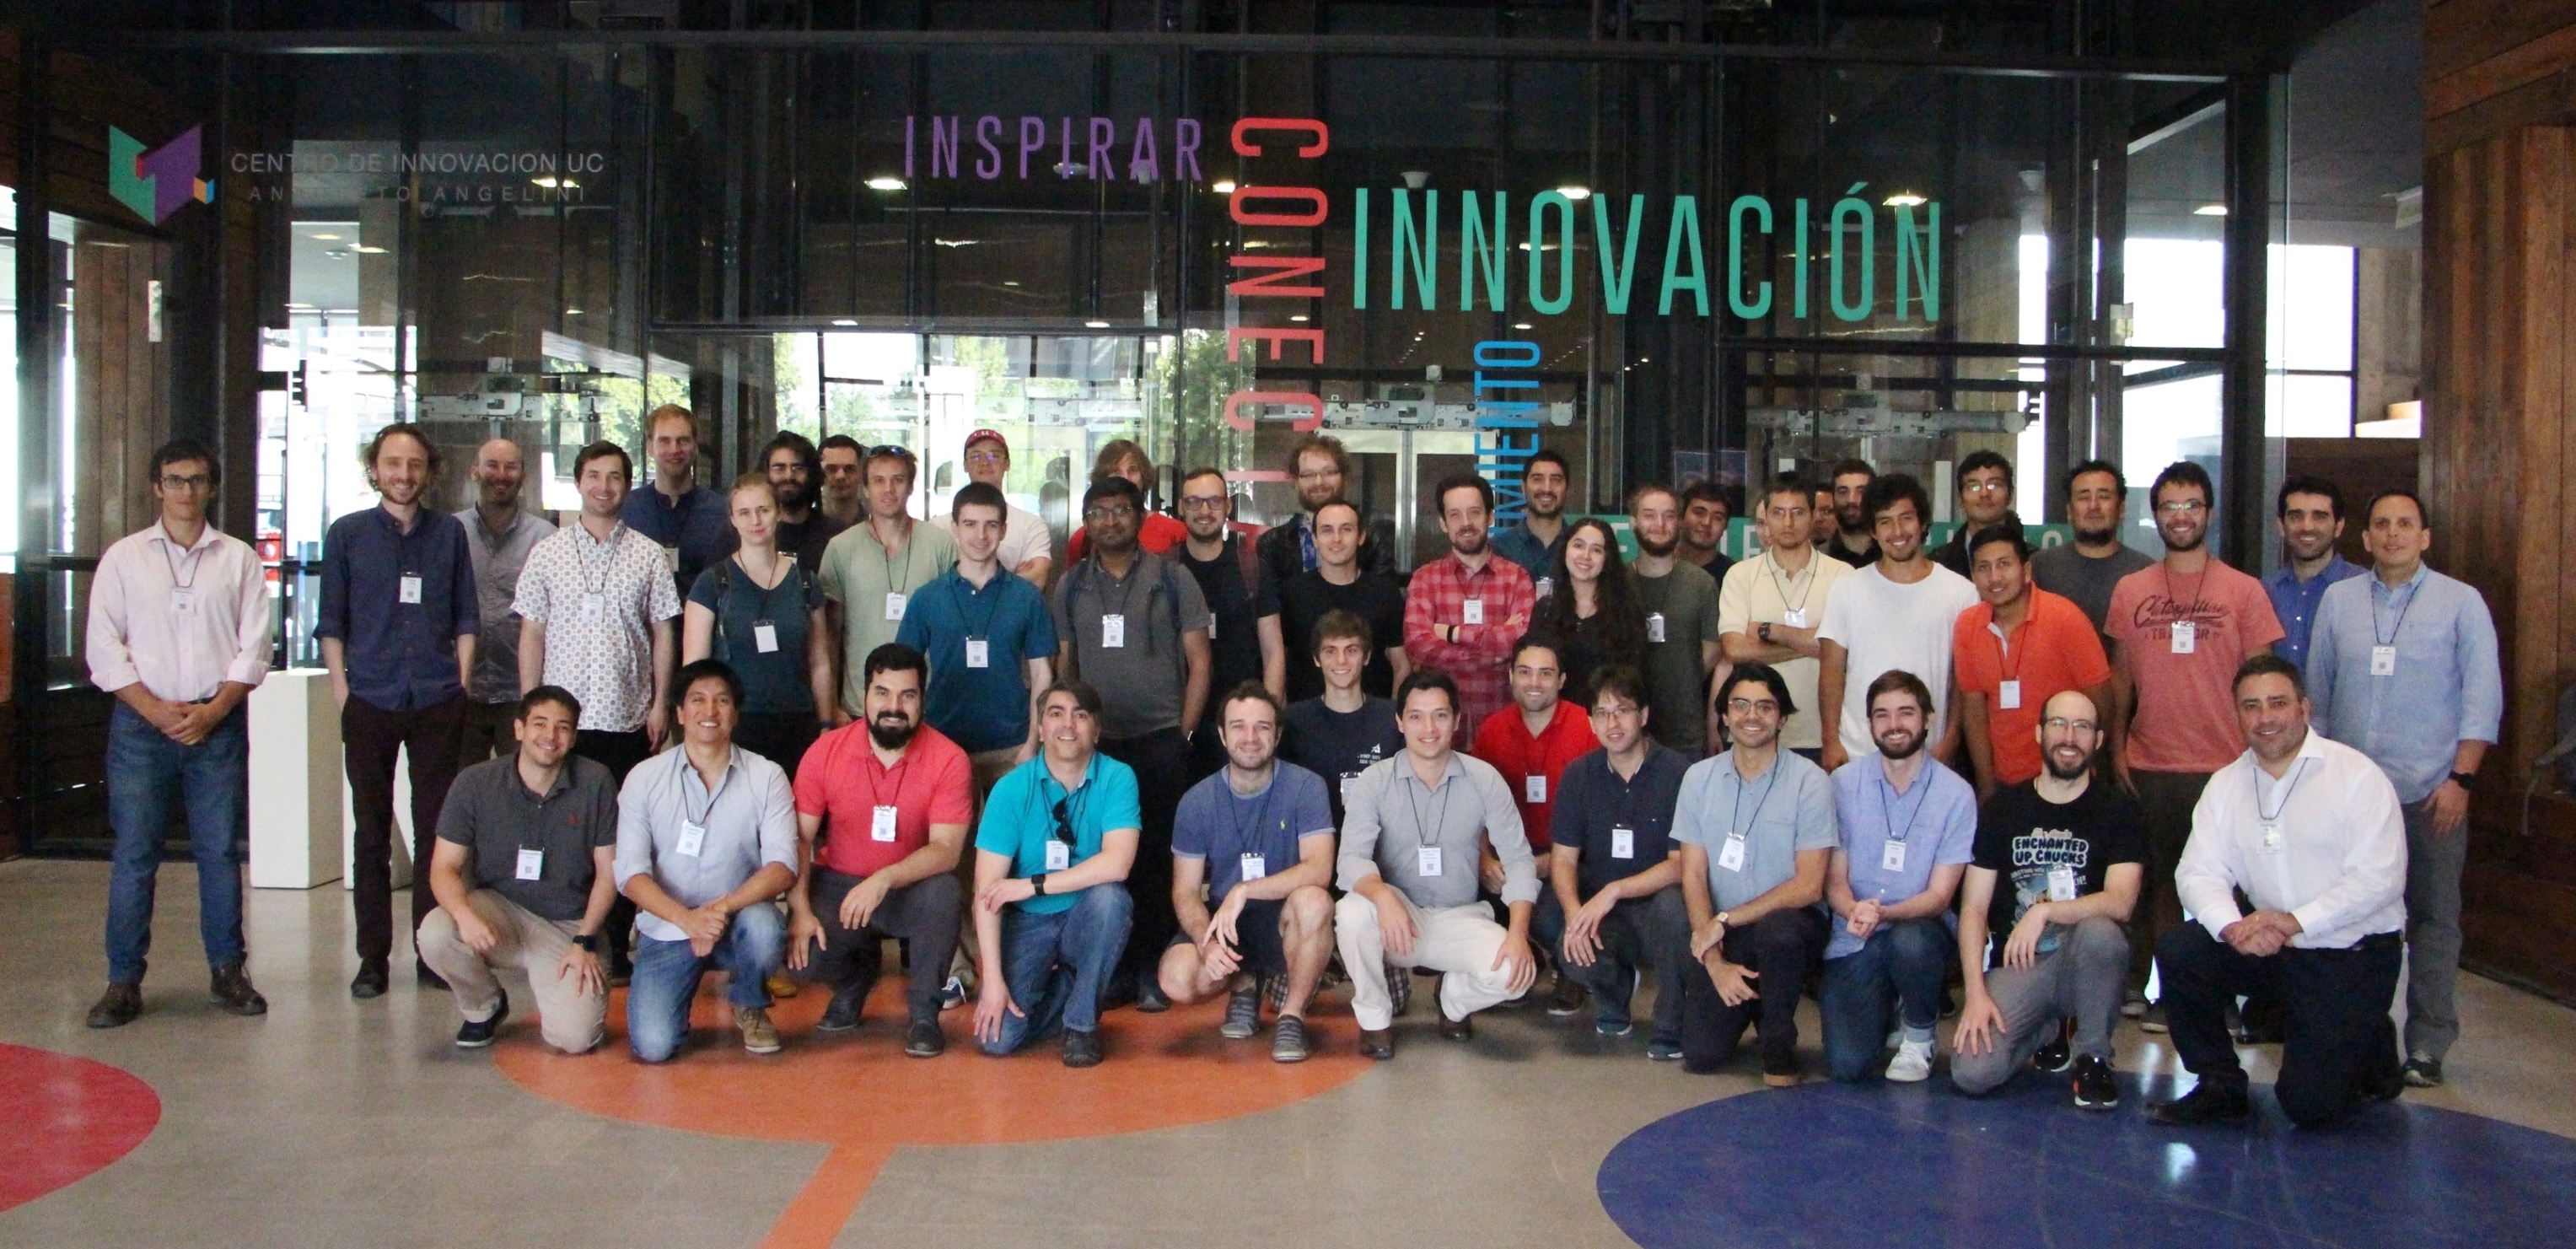
\includegraphics[width=0.8\textwidth]{../../latex/images/JuMP-dev_2019.jpeg}
  \end{center}
    \end{column}
    \begin{column}{0.5\textwidth}
  \begin{itemize}
    \item First at MIT in June 2017.
    \item Second at Bordeaux before ISMP in June 2018.
    \item Third in Chile in March 2019.
    \item Coming at \alert{UCLouvain} between 15th--19th of June 2020.
  \end{itemize}
  Videos from past years available on Youtube.
    \end{column}
  \end{columns}
\end{frame}


\end{document}
